\begin{exercisePage}[Komplexe Zahlen \& Differenzierbarkeit]
%
% Aufgabe 1.1
\begin{task} \label{task: 1.1}
	Wo liegen in der Gaußschen Zahlenebene diejenigen Punkte $z$, für die gilt
	\begin{enumerate}[leftmargin=*, nolistsep, topsep=-\parskip]
		\item $0 < \Re(\i z) < 2\pi$
		\item  $\abs{z - z_1} = \abs{z - z_2}$ ($z_1, z_2 \in \CC$ gegeben)
		\item $\abs{z} + \Re(z) < 1$
		\item $z^5 = 1$
		\item $z = 3 - \i + 5e^{\i t}$ ($0 \le t \le \pi$)
		\item $z = te^{\i t}$ ($t \ge 0$)
	\end{enumerate}
\end{task}

\begin{enumerate}[leftmargin=*, label=(zu \alph*)]
	\item Mit $z = a + b\i$ ist $\i*z = -b + a\i$, d.h. $\Re(\i * z) = - \Im(z)$.
	\item Der Term $\abs{z - z_1}$ beschreibt den Abstand zwischen $z$ und $z_1$, d.h.  $\abs{z - z_1} = \abs{z - z_2}$ beschreibt alle Punkte, die von $z_1$ und $z_2$ den gleichen Abstand haben. Dies sind alle Punkte, die auf der Geraden mit Normale $n = \quer{z_1z_2}$ liegen, d.h. $z$ erfülle die Bedingung $\scal{n}{\frac{1}{2} z_1 + \frac{1}{2} z_2 - z} = 0$, wobei $z, z_1, z_2$ als Punkte im $\R^2$ mit dem Standardskalarprodukt zu verstehen sind.
	\item Sei $z = a + b\i$, dann lässt sich die Gleichung schreiben als
	\begin{equation*}
		\begin{alignedat}{3}
			\sqrt{a^2 + b^2} + a &< 1 &\equivalent& &\sqrt{a^2 + b^2} &< 1 - a \\
			&&\equivalent& &a^2 + b^2 &< 1 - 2a + a^2 \\
			&&\equivalent& &y^2 &< 1 - 2x \\
			&&\equivalent& &\abs{y} &< \sqrt{1 - 2x} \\
			&&\equivalent& &-\sqrt{1 - 2x}  &< y < \sqrt{1 - 2x} 
		\end{alignedat}
	\end{equation*}
	Somit liegen alle gültigen $z$ in dem von einer nach links geöffneten Parabel mit Scheitelpunkt in $(\sfrac{1}{2}, 0)$ eingeschlossenen Bereich.
	\item Die Einheitswurzeln liegen stets auf dem Einheitskreis. Insbesondere bilden die fünften Einheitswurzeln ein Fünfeck, wobei ein Eckpunkt auf der Realachse liegt (da stets $1^5 = 1$). Außerdem lassen sich alle Lösungen dieser Gleichung explizit angeben mit
	\begin{equation*}
		z_k = \exp\brackets{\frac{2\pi \i * k}{5}} = \cos\brackets{\frac{2\pi * k}{5}} + \i * \sin\brackets{\frac{2\pi * k}{5}} \qquad (k = 0, 1 \dots, 4)
	\end{equation*}
	\item Wir schreiben $z= 3 - i +5e^{\i t} = 3 + 5 \cos(t) +\i * \brackets{5\sin(t) - 1}$. Damit erhalten wir eine Parameterdarstellung eines Kreises mit Radius $5$ und Zentrum $(3,-1)$. Da $t \in [0,\pi]$ liegen alle $z$ nur auf dem oberen Halbkreis.
	\item Der Ausdruck $r * e^{it}$ beschreibt einen Kreis mit Radius $r$ um den Ursprung. Da $t$ den Winkel zur Realachse beschreibt, wird der Radius von $t * e^{it}$ mit wachsendem Winkel größer, d.h. es ergibt sich eine (unendliche) Spirale.
\end{enumerate}

\begin{figure}
	\centering
	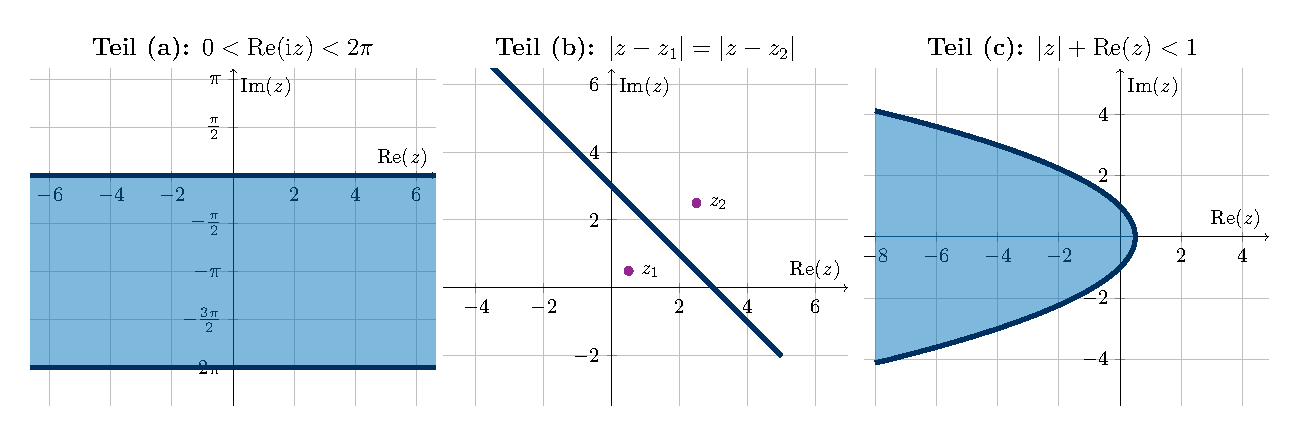
\includegraphics[width=\linewidth]{./fkt_uebungen-1-abb-abc.pdf}
	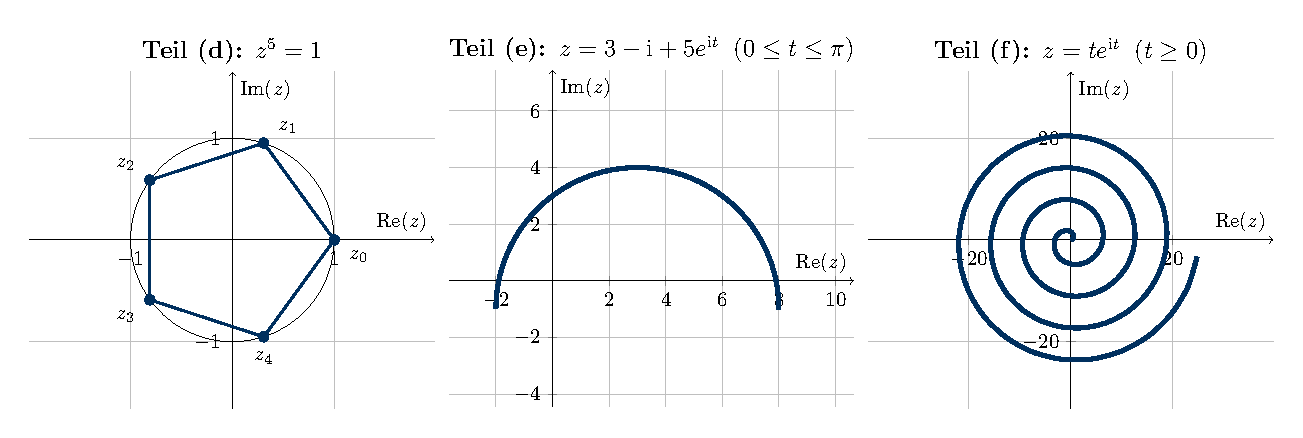
\includegraphics[width=\linewidth]{./fkt_uebungen-1-abb-def.pdf}
	\caption{Darstellungen zu \cref{task: 1.1}}
\end{figure}

\begin{task}
	Sei $\Omega \subseteq \CC$ offen, $z_0 \in \CC$, $\abb{f}{\Omega}{\CC}$.
	\begin{enumerate}[leftmargin=*, nolistsep, topsep=-\parskip]
		\item Zeigen Sie: $f$ ist genau dann in $z_0$ differenzierbar, wenn es $a \in \CC$ und $\abb{\phi}{\Omega}{\CC}$ mit $\lim_{z \to z_0} \phi(z) = 0$ gibt, sodass
		\begin{equation*}
			f(z) = f(z_0) + a (z-z_0) + \abs{z-z_0} \phi(z) \qquad (z \in \Omega)
		\end{equation*}
		gilt. Es ist dann $f'(z_0) = a$.
		\item Sei $\Omega' \subseteq \CC$ offen, $\abb{g}{\Omega'}{\CC}$, $f(\Omega) \subseteq \Omega'$ und seien $f$ in $z_0$ und $g$ in $f(z_0)$ differenzierbar. Zeigen Sie, dass $g \circ f$ in $z_0$ differenzierbar ist und dass
		\begin{equation*}
			(g \circ f)'(z_0) = g'(f(z_0)) * f'(z_0)
		\end{equation*}
		gilt (Kettenregel).
	\end{enumerate}
\end{task}

\pagebreak

\begin{enumerate}[leftmargin=*, label=(zu \alph*)]
	\item \begin{equivalence}
		\hinrichtung $f$ sei komplex differenzierbar in $z_0$, d.h. $f'(z_0)$ existiert. Definieren wir $a \defeq f'(z_0)$ und 
		\begin{equation*}
			\phi(z) \defeq \frac{z-z_0}{\abs{z-z_0}} * \schlange{\phi}(z) \quad \mit \quad  \schlange{\phi}(z) \defeq  \frac{f(z) - f(z_0)}{z-z_0} - f'(z_0)
		\end{equation*}
		Dann ist
		\begin{equation*}
			\begin{array}{rl}
			&f(z_0) + a(z-z_0) + \abs{z-z_0} \phi(z) \\
			=& 	f(z_0) + f'(z_0) * (z-z_0) + \abs{z-z_0} * \frac{z-z_0}{\abs{z-z_0}} * \brackets{\frac{f(z) - f(z_0)}{z-z_0}  - f'(z_0)}  \\
			=& f(z_0) + f'(z_0) * (z-z_0) + f(z) - f(z_0)  - f'(z_0) (z-z_0) \\
			=& f(z)
			\end{array}
		\end{equation*}
		Außerdem gilt aufgrund der Differenzierbarkeit von $f$ auch $\schlange{\phi}(z) \to 0$ für $z \to z_0$ sowie
		\begin{equation*}
			\abs{\frac{z-z_0}{\abs{z-z_0}}} = \frac{\abs{z-z_0}}{\abs{z-z_0}} = 1
		\end{equation*}
		und somit ist der Ausdruck $\frac{z-z_0}{\abs{z-z_0}}$ beschränkt. Schließlich dominiert somit $\schlange{\phi}$ die Konvergenz von $\phi$ und es gilt
		\begin{equation*}
			\lim_{z \to z_0} \phi(z) = 0
		\end{equation*}
		%
		\rueckrichtung Es existieren $a \in \CC$ und $\abb{\phi}{\CC}{\CC}$ mit $\phi(z) \to 0$ und $f(z) = f(z_0) + a * f'(z_0) (z-z_0) + \abs{z-z_0} * \phi(z)$. Daraus lässt sich umstellen
		\begin{align*}
				\frac{f(z) - f(z_0)}{z-z_0} 
				&= a + \phi(z) * \abs{z-z_0} * \frac{\quer{z-z_0}}{\quer{z-z_0}} \\
				&= a + \phi(z) * (z-z_0) * \frac{\quer{z-z_0}}{\abs{z-z_0}} \tag{$\frac{\abs{z}}{\quer{z}} = \frac{z}{\abs{z}}$}\\
				\follows \frac{f(z) - f(z_0)}{z-z_0} &= a + \phi(z) * \frac{\quer{z-z_0}}{\abs{z-z_0}}
		\end{align*}
		Somit ist 
		\begin{equation*}
			\lim_{z \to z_0} \frac{f(z) - f(z_0)}{z-z_0} = a + \lim_{z \to z_0} \underbrace{\phi(z) * \frac{\quer{z-z_0}}{\abs{z-z_0}}}_{\defqe \schlange{\phi}(z)}
		\end{equation*}
		Wie oben ist
		\begin{equation*}
			\abs{\frac{\quer{z-z_0}}{\abs{z-z_0}}} = \frac{\abs{z-z_0}}{\abs{z-z_0}} = 1
		\end{equation*}
		und somit dominiert $\phi$ den Ausdruck $\schlange{\phi}$ zu Null, d.h.
		\begin{equation*}
			\lim_{z \to z_0} \frac{f(z) - f(z_0)}{z-z_0} = a + \lim_{z \to z_0} \schlange{\phi}(z) = a \follows a = f'(z_0)
		\end{equation*}
	\end{equivalence}
	%
\pagebreak
	%
	\item Es seien $\abb{f}{\Omega}{\CC}$ in $z_0$ und $\abb{g}{\Omega'}{\CC}$ in $f(z_0)$ komplex differenzierbar.
	Dann gilt
	\begin{align*}
			\lim_{z \to z_0} \frac{(g \circ f) (z) - (g \circ f)(z_0)}{z - z_0}
			&= \lim_{z \to z_0} \frac{(g \circ f) (z) - (g \circ f)(z_0)}{f(z) - f(z_0)} * \frac{f(z) - f(z_0)}{z - z_0} \\
			&= \lim_{z \to z_0} \frac{(g \circ f) (z) - (g \circ f)(z_0)}{f(z) - f(z_0)} * \lim_{z \to z_0} \frac{f(z) - f(z_0)}{z - z_0} \\
			&= g'(f(z_0)) * \lim_{z \to z_0} \frac{f(z) - f(z_0)}{z - z_0} \tag{$g$ diffbar in $f(z_0)$} \\
			&= g'(f(z_0)) * f'(z_0) \tag{$f$ diffbar in $z_0$} 
	\end{align*}
	Insbesondere existieren die Grenzwerte $\lim_{z \to z_0} \frac{(g \circ f) (z) - (g \circ f)(z_0)}{f(z) - f(z_0)}$ und $\lim_{z \to z_0} \frac{f(z) - f(z_0)}{z - z_0}$ und somit auch der Grenzwert $\lim_{z \to z_0} \frac{(g \circ f) (z) - (g \circ f)(z_0)}{z - z_0}$, d.h. $g \circ f$ ist komplex differenzierbar in $z_0$.
\end{enumerate}

\begin{task}
	Seien $\abb{f,g,h}{\CC}{\CC}$ definiert durch
	\begin{equation*}
		\begin{aligned}
		f(z) &\defeq x^2 + y^2 \\
		g(z) &\defeq 2xy + y + \i (x^2 - y^2 - x) \\
		h(z) &\defeq \frac{x - \i y}{1 + x^2 + y^2}
		\end{aligned}
	\end{equation*}
	Bestimmten Sie die Punkte in $\CC$, in denen $f$, $g$ und $h$ komplex differenzierbar sind.
\end{task}

Wir zerlegen die Funktionen immer in Real- und Imaginärfunktion, d.h. $f(z) = f(x,y) = f_1(x,y) + \i * f_2(x,y)$. Damit ist $f_1(x,y) = x^2 + y^2$ und $f_2(x,y) = 0$. Für die partiellen Ableitungen gilt
\begin{align*}
	\partial_x f_1(x,y)  &= 2x 	&	\partial_y f_1(x,y) &= 2y \\
	\partial_x f_2(x,y)  &= 0 	&	\partial_y f_2(x,y) &= 0
\end{align*}
Alle partiellen Ableitungen sind stetig, somit ist $\abb{f}{\R^2}{\R^2}$ (reell) differenzierbar. Wir prüfen die Cauchy-Riemann-Differentialgleichungen:
\begin{equation*}
	\begin{array}{rcrcrcrcrcr}
	\partial_x f_1(x,y) &=& \partial_y f_2(x,y) &\equivalent& 2x &=& 0 &\equivalent& x &=& 0 \\
	\partial_y f_1(x,y) &=& - \partial_x f_2(x,y)  &\equivalent& 2y &=& 0 &\equivalent& y &=& 0 
	\end{array}
\end{equation*}
Damit sind die beiden Gleichungen nur für $z = 0$ erfüllt und $f$ ist nur in diesem Punkt komplex differenzierbar.

Es ist $g_1(x,y) = 2xy + y$ und $g_2(x,y) = x^2 - y^2 - x$. Für die partiellen Ableitungen gilt
\begin{align*}
	\partial_x g_1(x,y)  &= 2y 		&	\partial_y g_1(x,y) &= 2x+1 \\
	\partial_x g_2(x,y)  &= 2x-1	&	\partial_y g_2(x,y) &= -2y
\end{align*}
Alle partiellen Ableitungen sind stetig, somit ist $\abb{f}{\R^2}{\R^2}$ (reell) differenzierbar. Wir prüfen die Cauchy-Riemann-Differentialgleichungen:
\begin{equation*}
\begin{array}{rcrclclcrcr}
	\partial_x g_1(x,y) &=& \partial_y g_2(x,y) &\equivalent& 2y &=& -2y &\follows& y &=& 0 \\
	\partial_y g_1(x,y) &=& - \partial_x g_2(x,y)  &\equivalent& 2x+1 &=& -2x+1 &\follows& x &=& 0 
\end{array}
\end{equation*}
Damit sind die beiden Gleichungen nur für $z = 0$ erfüllt und $g$ ist nur in diesem Punkt komplex differenzierbar.

Es ist $h_1(x,y) = \frac{x}{1 + x^2 + y^2}$ und $h_2(x,y) = - \frac{y}{1 + x^2 + y^2}$. Für die partiellen Ableitungen gilt
\begin{align*}
	\partial_x h_1(x,y)  &= \frac{1-x^2+y^2}{(1 + x^2 + y^2)^2}	&	\partial_y h_1(x,y) &= \frac{-2xy}{(1 + x^2 + y^2)^2} \\
	\partial_x h_2(x,y)  &= \frac{-2xy}{(1 + x^2 + y^2)^2}		&	\partial_y h_2(x,y) &= -\frac{1+x^2-y^2}{(1 + x^2 + y^2)^2}
\end{align*}
Alle partiellen Ableitungen sind stetig für $x \neq \pm \sqrt{-y^2-1}$, somit ist $\abb{f}{\R^2}{\R^2}$ dort (reell) differenzierbar. Wir prüfen die Cauchy-Riemann-Differentialgleichungen:
\begin{equation*}
\begin{array}{rcrcccrcl}
	\partial_x h_1(x,y) &=& \partial_y h_2(x,y) &\equivalent& \frac{1-x^2+y^2}{(1 + x^2 + y^2)^2} = -\frac{1+x^2-y^2}{(1 + x^2 + y^2)^2} &\follows& 1 &=& -1 \\
	\partial_y h_1(x,y) &=& - \partial_x h_2(x,y)  &\equivalent& \frac{-2xy}{(1 + x^2 + y^2)^2} = \frac{2xy}{(1 + x^2 + y^2)^2} &\follows& -2xy &=& 2xy
\end{array}
\end{equation*}
Die erste Gleichung liefert aufgrund der falschen Aussage für alle $x,y \in \R$ die Unlösbarkeit des Gleichungssystems. Somit ist $h$ nirgends komplex differenzierbar.

\end{exercisePage}